\documentclass[a4paper,11pt,fleqn]{article}%fleqn pour aligner les equations à gauche
\usepackage{../../Styles/Exercice}


\newcommand{\chnum}{Chapitre 18}
\newcommand{\chtitle}{Phénomènes ondulatoires}
\newcommand{\dtype}{Exercices}
  
\begin{document}
\maketitle

\begin{multicols}{2}
\section{Périodicité d'une onde}
Une onde mécanique progressive sinusoïdale de fréquence $f$ = \num{1,5} \unit{\mega\hertz} et de phase à l'origine $\phi = \dfrac{\pi}{2}$ se propage avec une célérité $c$ = \num{1500} \unit{\meter\per\second}.
\begin{itemize}
    \item Déterminer la période $T$ ainsi que la longueur d'onde $\lambda$ de l'onde mécanique.
\end{itemize}

\section{Identification d'une onde sinusoïdale}
L'amplitude d'une onde mécanique est modélisée par la fonction suivante :
\begin{eqnarray}
s(x,t)=2,0 \times \cos{\left( \dfrac{2\pi}{2,0 \times 10^{-3}} \times \left( t - \dfrac{x}{c}\right) + \dfrac{\pi}{3}\right)} \nonumber
\end{eqnarray}
\begin{enumerate}
    \item À partir de l'expression ci-dessus, déterminer la valeur de la période $T$ et de la phase à l'origine $\phi$.
    \item Déterminer la valeur de l'amplitude $s$ de l'onde à l'origine ($x$ et $t$ sont nuls).
    \item À $x$ = \num{0} \unit{\meter}, représenter graphiquement l'évolution de l'amplitude de l'onde $s(x,t)$ sur une durée égale à $3T$ à la calculatrice.
    \item Sur le même graphique, représenter une onde identique mais dont le déphasage à l'origine est égal à zéro.
\end{enumerate}

\section{Expérience d'Young}
Thomas Young élabore en 1801 un dispositif pour démontrer la nature ondulatoire de la lumière. Cette expérience est restée célèbre sous le nom d'expérience des trous d'Young. Vers 1818, le français Augustin Fresnel a l'idée de remplacer les trous par des fentes.
\begin{itemize}
    \item Parmi les trois photographies ci-dessous, identifier celles qui correspondent aux deux expériences décrites dans l'énoncé. Justifier.
\end{itemize}
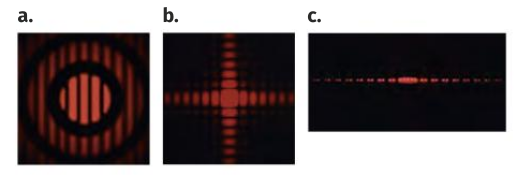
\includegraphics[scale=.7]{Ressources/TSPE_C9_Exercices_Fig1.png}

\section{Interférence sonore}
Une vidéo a créé le \emph{buzz} en montrant un appareil capable d'annuler le bruit venant de l'extérieur d'un appartement en le ventousant simplement sur le fenêtre. Si cette technologie existe pour les casques audio à réduction active de bruit, qu'en est-il pour une pièce entière ?
\begin{enumerate}
    \item Nommer le phénomène sur lequel repose le principe de fonctionnement des casques à réduction active de bruit.
    \item Schématiser simplement le principe physique de fonctionnement d'un tel appareil.
\end{enumerate}

\section{Diffraction à la surface de l'eau}
L'image ci-dessous est la photographie de la propagation d'ondes progressives périodiques à la surface de l'eau dans une cuve  à ondes. Les ondes se propagent vers la droite.
\begin{enumerate}
    \item Expliquer ce que cette expérience illustre.
    \item Comparer les dimensions de l'ouverture de l'obstacle avec la longueur d'onde.
    \item Préciser comment évolue la longueur avant et après le passage de l'onde par l'ouverture.
\end{enumerate}
\begin{center}
	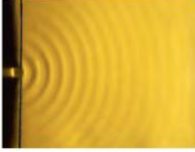
\includegraphics[scale = 1.5]{Ressources/TSPE_C9_Exercices_Fig2.png}
\end{center}

\section{Bulles de savon}
Lorsqu'un faisceau de lumière passe d'un milieu transparent, homogène et isotrope à un autre, une partie du faisceau est réfléchie, l'autre est réfractée. Les angles sont liés aux lois de Snell-Descartes.\\
Localement, une bulle de savon est modélisée comme une fine couche d'un matériau transparent entourée de deux autres milieux transparents d'indices différents. La différence de chemin optique $\delta$ entre le  rayon 1 et le rayon 2 ne dépend que de l'épaisseur $e$, de l'indice de réfraction $n$, de l'angle de réfraction $\beta$ et de la longueur d'onde $\lambda$ du faisceau incident :$$ \delta = 2 n \cdot e \cdot \cos(\beta) + \dfrac{\lambda}{2} $$
\begin{center}
    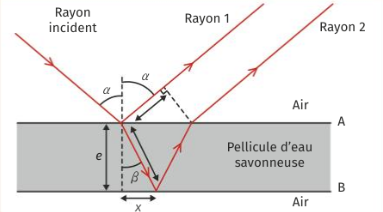
\includegraphics[scale = .95]{Ressources/TSPE_C9_Exercices_Fig3.png}
\end{center}

    \begin{enumerate}
    \item Exprimer la différence de chemin optique dans les cas d'interférence constructives et destructives.
    \item On considère que l'observation se fait sous incidence normale ($\beta$ = 0 \unit{\radian}). Pour chacune des situations précédentes, établir l'expression de l'épaisseur $e$ du film d'eau savonneuse en fonction de $n$, $\lambda$ et $k$ (l'ordre d'interférences).
    \item Pour l'intervalle en longueur d'onde du domaine du visible [\SI{400}{\nano\meter} ; \SI{800}{\nano\meter}] et un indice de réfraction $n$ = \num{1,34}, calculer les épaisseurs $e$ du film dans les cas d'interférences constructives et destructives d'ordre 1 ($k$ = 1).
    \item Quand l'épaisseur $e$ du film devient supérieure à \SI{30}{\nano\meter}, plusieurs longueurs d'onde interfèrent. Pour une épaisseur de \SI{900}{\nano\meter}, déterminer les couples de valeurs $k$ et $\lambda$ pour lesquels des interférences constructives sont attendues. En déduire la couleur des franges.
    \item Une zone blanche apparaît avant l'éclatement du film d'eau savonneuse. Expliquer pourquoi.
\end{enumerate}
\begin{center}
    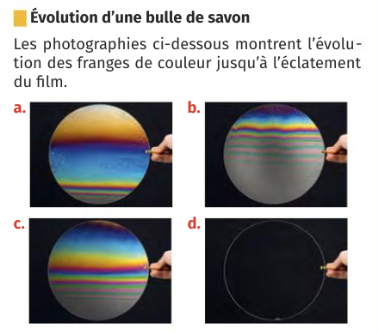
\includegraphics[scale = .95]{Ressources/TSPE_C9_Exercices_Fig4.png}
\end{center}

\section{Interféromètre de Michelson}
De nos jours, l'interféromètre de Michelson peut être utilisé pour mesurer avec précision la longueur d'onde d'une source lumineuse monochromatique.\\
Un faisceau de lumière issu d'une source laser est séparé en deux au point $A$ d'une lame séparatrice semi-réfléchissante. Chacun des deux faisceaux ainsi formés est alors en phase. Ils constituent un système de deux sources cohérentes.\\
Ces deux faisceaux sont réfléchis par des miroirs plans $M_1$ et $M_2$ (respectivement aux points $B$ et $C$) et redirigés vers le point $A$ de la lame séparatrice pour finalement se rejoindre au niveau d'un capteur qui mesure l'intensité lumineuse résultante.\\
L'un des miroirs (le miroir $M_1$ par exemple) est placé sur un chariot motorisé afin de le faire glisser lentement et de façon continu. Le mouvement du chariot modifie le trajet de l'un des faisceaux, modifiant l'intensité lumineuse mesurée par le capteur : on observe une alternance d'interférences constructives et destructives.
\begin{center}
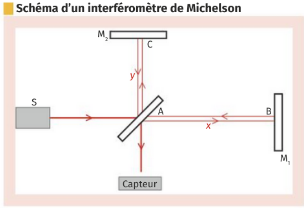
\includegraphics{Ressources/TSPE_C9_Exercices_Fig5.png}
\end{center}
\begin{enumerate}
    \item Exprimer la différence de chemin optique $\delta$ entre les deux faisceaux en fonction des distances $x$ et $y$.
    \item Lorsque $x=y$, préciser ce qu'enregistre le capteur.
\end{enumerate}
Quand le chariot démarre et s'arrête, le capteur enregistre une intensité maximale. Pendant le déplacement d'une distance $d$ du miroir $M_1$ le capteur a enregistré une alternance de 6522 plages sombres.
\begin{enumerate}[resume]
    \item Donner l'expression de la différence de chemin optique $\delta$ en fonction de $d$.
    \item Donner l'expression de la différence de chemin optique $\delta$ en fonction de la longueur d'onde dans le cas d'interférences constructives.
    \item En déduire la longueur d'onde $\lambda$ du laser pour un déplacement $d$ = \SI{2,064}{\milli\meter} du miroir.
\end{enumerate}
\end{multicols}
\end{document}